\chapter{Research}
\label{Chapter:Research}
Social media sites have become integral to daily life in today's society. It is difficult for new ideas to gain popularity and draw users from their established social networks. Even for social media juggernauts like Facebook and Twitter, user retention is a challenge currently being faced. This has driven the need for the addition of innovative features to existing systems, such as the ability to use virtual reality headsets for viewing images and videos \cite{Facebook:VR}. To be able to achieve the goals set out for Fidelis, it was imperative to look at existing systems and build on what they have done successfully, but also identify their downfalls and improve upon these. Additionally, research into a number of techniques that can address these downfalls and provide Fidelis users with security and comfort was conducted.

\section{Related Work}
The following sections will discuss the research pursued on the four core Fidelis functionalities: abuse detection, content filtering, content recommendation and reputation scoring. Each section considers the aforementioned topic and looks at a number of different approaches for each of them.

\subsection{Abuse Detection}
Basic abuse detection on social media platforms consists of rudimentary techniques such as flagging content deemed offensive or through the existence of content moderators. However, for more advanced methods most abuse detection systems employ natural language processing (NLP) and machine learning techniques to detect abusive user content. It is common to build a machine learning model that has the ability to classify content as abuse or not. For the purposes of this report, we will focus on user posts on a social media site. Classifiers learn from a given collection of abusive posts and use the resulting model to classify future posts. There is variation in the features extracted from posts to be used for training models. The success and accuracy of classifiers hinge very much on the selected features, making feature selection an important part of building the classifier.

As with any system that attempts NLP, the difficulty in detecting abusive posts lies within the intricacies of the English language. The task of identifying abusive content is unfortunately not as simple as a keyword search and needs some understanding of underlying language structure and consideration for its linguistic features. As identified by Nobata et al in their research, \cite{nobata2016abusive}, when abusive language is used online it is purposefully obfuscated to lessen the chance of it being detected. This, coupled with the seemingly popular use of ``text speech'' makes the simple task of detecting `\emph{sh*t}' much harder when a system faces (arguably) creative variations like `\emph{sh*eeeeeet}'. Abuse obfuscation also does not necessarily have to focus on the word itself, but can instead be hidden in the delivery of the message. Perfect grammar and spelling can be used just as effectively, if not more, to mask the true meaning behind a message. This again highlights the inefficacy in just using keywords. Challenges faced when detecting abuse are not only from correctly identifying abusive posts, but are also from avoiding the misclassification of non-abusive posts. Profanity can be used for abuse, emphasis, playfulness or frustration. We are only interested in profanity being used for abuse, and as such the remaining use cases need not be detected. 

Features commonly extracted from natural language to perform abuse detection are syntactic and lexical features. Syntactic features look at words alone and explore the relationship between words in a sentence \cite{liao2010large}. This can be seen in part-of-speech tagging, which tags a word in a sentence based on its syntactic class. Words in different contexts would be tagged differently, which leads to dis-ambiguity when processing words. Using syntactic features, we can identify the relationship between \emph{he} and \emph{dog} in the following sentence:

\begin{equation}
\label{eq:semantic}
\mbox{\textsl{The dog ran after the ball; he really enjoyed playing games with his owner.}}
\end{equation}

Comparatively, lexical features treat each word or phrase as an individual entity, meaning word patterns can be found in sentences by the appearance of words and their frequencies \cite{chen2012detecting}. An example lexical feature is the stemmed version of a word. Stemming reduces all occurrences of words to their ``root'' word \cite{Elastic:Stem}. So in the above example, the root for \emph{enjoyed} would be \emph{enjoy}. 

In their work on an abuse detection classifier, Nobata et al \cite{nobata2016abusive} use syntactic and lexical features, in addition to n-gram, linguistic and distributional semantic features. 3-5 character n-grams are used to identify abusive language that has been obfuscated by elongating the original word (\textsl{lol} becomes \textsl{looooool}). Whereas n-gram features are used to detect directly abusive words, syntactic features are used to capture long-range dependencies between words using dependency parsing. Through the combination of these features, the resulting classifier is able to detect hate speech, derogatory and profane language.

Ravazi et al built an automatic flame detection system \cite{razavi2010offensive}, where content is deemed `flame' if its main intention is to attack (hate speech, racism, extremism, homophobia) or it contains abusive or hostile words, phrases or language. The system is built upon a three-level classifier. Each level extracts a set of features which are then used as the input for the next level. The first level uses the Complement Naive Bayes classifier to select the most discriminative features. The second level uses the Multinomial Update Naive Bayes Classifier. The third and final level uses DTNB, which is a rule-based classifier. The third level also makes use of an Insulting and Abusing Language Dictionary, which is a collection of words, phrases, and expressions, with different degrees of manifestation of flame varieties.

More recently, Chatzakou et al looked at identifying bullies and aggressive users on Twitter by characterising users based on user, text and network-based features \cite{chatzakou2017mean}. Focusing on just the text-based features, word embeddings were used to capture the syntactic and semantic relations in words. In their works, the word2vec model developed by Mikolov et al \cite{mikolov2013efficient}, is used to generate a vector representation for a given post, which it gets by averaging the vectors for each word in the post. This is coupled with the use of the SentiStrength tool \cite{SentiStrength:Home}, which estimates the positive and negative sentiment in short texts. These features alone would not suffice for abuse detection but combined with user and network-based features provide a new and innovative way of approaching the problem of abusive language detection.

\subsection{Content Filtering} \label{sec:research-content-filtering}
As with the abuse detection, content filtering is a classification problem. Classification in this instance, however, is concerned with the automated categorisation of users posts. Each post is assigned to a topic based on its content. These categorised posts enable output to be presented to users as a set of filtered feeds, making it easier for them to locate content they find engaging. Akin to abuse detection, content filtering requires NLP, which presents challenges when selecting an appropriate machine learning model to be used as the classifier, along with determining features to use for model training.

Before considering the type of model to use, feature extraction must be used to represent posts in a way which allows a model to detect patterns. The most common method of feature extraction technique for textual content is the Bag-of-Words (BoW) representation, whereby ``a document is considered to be simply a collection of the words which occur in it at least once. The order of the words, the combinations in which they occur, paragraph structuring, punctuation and of course the meanings of the words are all ignored''~\cite{Bramer:BoW}. The loss of ordering in the content can result in some of the meaning of the post being lost. Despite this, ``BoW features are effective at capturing the general topic of the discourse in which the topic had occurred''~\cite{Jurafsky:BoW}.

With regards to the model itself, there are numerous models which perform classification, including Na\"ive Bayes, Support Vector Machines (SVMs) and k-Nearest Neighbours, with each model having its own advantages and disadvantages.

Na\"ive Bayes assumes that each feature in the data is independent in order to calculate the maximum posterior given the training data~\cite{Kuncheva:Bayes}. This is done by maximising the Bayes formula, where $c$ is the number of classes and $i$ is each possible model:

\begin{equation}
\label{eq:bayes}
P(\omega_{i}|\mathbf{x}) = \frac{P(\omega_{i})p(\mathbf{x}|\omega_{i})}{\sum_{j=1}^{c}P(\omega_{j})p(\mathbf{x}|\omega_{j})}\quad i=1,...,c
\end{equation}

\noindent Using the Na\"ive Bayes assumption of independence, we can simplify the above formula to:  
\begin{equation}
\label{eq:bayes-simple}
p(\mathbf{x}|\omega_{i})=\prod_{j=1}^{n}p(x_{j}|\omega_{i})\quad i=1,...,c
\end{equation}

\noindent ,where $n$ is the number of inputs. This simplification makes computation inexpensive, but the assumption may not necessarily hold with the posts on Fidelis. For example, the presence of one word in the BoW could increase the likelihood of another word being present, thus assuming independence may make the model less effective.

Conversely, SVMs uses a decision boundary to categorise data. The boundary ``is chosen to be the one for which the margin is maximized''~\cite{Bishop:SVM}, where the margin is the distance between the boundary and the nearest data points from each class. One possible difficulty with using SVMs is the choice of kernel, which is used to measure the similarity of two data points. This is because ``once the kernel is fixed, SVM classifiers have only one user-chosen parameter (the error penalty), but the kernel is a very big rug under which to sweep parameters''~\cite{Burges:SVM}.

k-Nearest Neighbours ``directly uses the data sample to estimate the density''~\cite{Zaki:KNN}. The performance of this model decreases as the dimensionality of the data increases, so due to the likely sparsity of the data which the model will be using in Fidelis, this could have a major implication on the effectiveness of the topic categorisation. Another drawback is that the use of k-Nearest Neighbours is ``computationally expensive''~\cite{Kuncheva:KNN}.

Since Fidelis will be required to categorise posts from the launch of the site, even when no posts currently exist, data must be collected from existing social media platforms, which can model realistic Fidelis posts. These posts must also be assigned to a category, enabling a classifier to be trained on the data collected. As part of their paper Zubiaga and Ji curated a set of tweets which were assigned one of the following categories: arts, business, education, games, health, home, news, recreation, science, shopping, society, sport and technology \cite{Zubiaga:Tweets}. The dataset has been made publicly available so can be used to train the classifier.

\subsection{Content Recommendation}
As previously mentioned, the public is demanding more from social media platforms in terms of how they interact with and are engaged by the network. In recent years there has been a welcomed increase in the application of recommender systems. Recommender systems provide item recommendations that might be of interest to a user \cite{ricci2011introduction}. Originally used on music and video streaming services like Spotify and Netflix, recommender systems have permeated to social media platforms. The challenge faced when recommending new items to a user is that there is no guarantee that the user will like the content. Research has therefore focused on tailoring and personalising recommendations to a given user. To this end, most recommender systems implement either content or collaborative-based filtering algorithms.

\subsubsection{Collaborative-based Filtering} 
With collaborative-based filtering algorithms, users are recommended new content based on the opinion of other like-minded users or using information from content previously rated by the user \cite{sarwar2001item}. Recommendations take the form of either predictions, which are numerical values that represent how likely it is for the user to like an item they have not previously liked, or as a list of $N$ items the user will like the most \cite{sarwar2001item}. Such algorithms can be memory-based, building a network of neighbours around the user who have a history of agreeing with them \cite{sarwar2001item}, or model-based, whereby a machine learning approach is taken and item recommendations are viewed probabilistically. A common approach to collaborative-based filtering is to build an $N \times N$ user similarity matrix. Each entry in the matrix corresponds to the similarity score between user $u_i$ and $u_j$. This is illustrated in equation \ref{example:similarity-matrix} for a system with three users. 

\begin{equation}
\bordermatrix{~ & u_1 & u_2 & u_3 \cr
            u_1 & - & 0.76 & 0.83 \cr
            u_2 & 0.76 & - & 0.6\cr
            u_3 & 0.83 & 0.6 & - \cr}
\label{example:similarity-matrix}
\end{equation}

User similarities are calculated using a number of different methods, but the preferred similarity measure is cosine similarity \cite{linden2003amazon, sarwar2001item, liu2014new}. Other similarity measures used include mean square difference (equation \ref{eq:msd}) and Jaccard similarity (equation \ref{eq:jacard}) \cite{liu2014new}. The similarity between users is determined by each users item-vector.

\begin{align}
msd(\mathbf{A}, \mathbf{B}) = \frac{1}{N}\sum\limits_{i=1}^{n}(A_i - B_i)^2 \label{eq:msd} \\
jacard(\mathbf{A}, \mathbf{B}) = \frac{\mathbf{A} \cdot \mathbf{B}}{\|\mathbf{A}\|^2 + \|\mathbf{B}\|^2 -  \mathbf{A} \cdot \mathbf{B}} \label{eq:jacard}
\end{align}
Vectors are created from items rated by the user, allowing the similarity between two vectors to be measured. Item-based collaborative filtering can be used as a replacement for user-based filtering. This variant on collaborative filtering provides recommendations based on item similarities. Items that a user has previously rated are scored against ``unseen'' items, and the user is presented with a list of the top $N$ recommendations \cite{sarwar2001item}. Similarity can  again be determined using either cosine or conditional probability-based calculations. Alternatively, with conditional probability-based similarity two items are similar if the probability that a new item will be consumed given another item already consumed by the user is high \cite{sarwar2001item}. The conditional probability is calculated based on the frequency of an item, where frequency for an item $X$ is the number of users that have consumed or rated $X$. 

\subsubsection{Content-based Filtering} 
Content-based filtering algorithms measure the correlation between the content of ``candidate'' recommendation items and items previously rated by the user \cite{van2000using}. This is the only major difference between the two filtering approaches. Similarly to collaborative-based filtering, the similarity between a ``candidate'' item and a user is calculated using the same similarity measures, and again using a vector of features for a given item. Features composing each item vector vary, but common techniques to extract textual features include:
\begin{itemize}
\item Bag of Words (BoW), which is discussed in earlier in chapter \ref{sec:research-content-filtering}
\item Term Frequency-Inverse Document Frequency (TF-IDF) \cite{van2000using}, where terms (or words) are assigned a weight based on how often they appear in a particular document and how frequently they occur across the entire collection of documents \cite{scikit:tfidf}
\end{itemize} 

\subsection{Reputation Scoring}
The concept of trust is imperative across all social networks. Different networks choose to model user trust in varying ways, with some networks choosing to follow an explicit trust model (if user A trusts user B, B also trusts A), and others preferring an implicit model (user A can trust User B, but trust is not necessarily reflexive). With regards to Fidelis, trust will be based upon reputation scores for both users and the posts they make. Having these scores attached to each user on the network will allow users to make informed decisions on who they choose to engage with. By building a circle of trust around themselves, users will be able to create a network of others with whom they can reliably engage with.

One interesting way to explore the idea of reputation scoring is through the use of collaboration-based reputation. In their paper, McNally et al explore the idea of modelling user reputations through collaboration events \cite{mcnally2013}. Collaboration events occur when users provide feedback on the content posted by other users. This feedback, for example in the form of voting on a post, is used in a calculation to determine how much the user giving feedback trusts the original poster. From these collaboration events, a collaboration graph can be created where nodes in the graph correspond to the original poster and users who provided feedback on the post. Trust scores are represented as edges in the graph and are aggregated to calculate the reputation of individual users using ``Weighted-Sum'' and ``Page Rank'' scoring metrics \cite{mcnally2013}.

Zacharia et al explore the application of collaborative reputation mechanisms used in electronic markets for wider use. Two mechanisms for scoring user reputations are discussed which can handle both loosely and highly connected online communities. The first, Sporas \cite{zacharia2000}, handles scoring reputations in a loosely connected community. Under Sporas, users have a single reputation which is updated according to feedback provided by other users. New users start with the minimum reputation value, and as a users' reputation grows they experience smaller changes in their reputation after each update. The second mechanism, Histos \cite{zacharia2000}, is a pairwise rating system. These pairwise ratings between users are modelled through a directed graph, with nodes in the graph representing users and ``weighted edges between nodes representing the most recent reputation given by one user to another, with the arrow pointing towards the rated user.'' \cite{zacharia2000}.

\section{Existing Systems}
There is a range of existing systems which provide a similar service or a subset of the services described in the project aims. However, these solutions have all been designed to tackle different problems and all have their respective drawbacks. In order to avoid facing problems that have been solved by these services, an analysis is carried out to discuss the advantages and shortcomings of each service. Using this, a superior social network which implements the advantages of these services whilst tackling the disadvantages can be designed.

\subsection{Facebook}
``Founded in 2004, Facebook's mission is to give people the power to share and make the world more open and connected''~\cite{Facebook:About}. Since its launch, it has become one of the most popular social networks to date and boasts an active user base of approximately 1.7 billion people \cite{Statista:Facebook}. According to Facebook, people use the social network ``to stay connected with friends and family, to discover what's going on in the world, and to share and express what matters to them''. Facebook users must register before using the social network and are free to create a personal profile in order to interact with other users who they can add as friends. Furthermore, Facebook users may join user groups based on workplace, college or school and can also categorise their Facebook contacts into lists. Users can post status updates or other content and message each other~\cite{Statista:Facebook}. 

The Facebook friend system operates on a mutual trust basis. This means if user A and user B are friends on Facebook because user A wishes to see content from user B then user B implicitly trusts user A and also sees content from user A. However, Facebook later realised that mutual trust does not imply friendship and added a following and unfollowing feature. As of this update, if two users are friends then they are automatically following each other but they can optionally unfollow one another, meaning that they will still have a friendship but will not see content from one another. This adds the concept of a one-way trust relationship which Fidelis aims to implement on an explicit level, which the user has control over and also on an implicit level, where content is filtered automatically through the use of reputation scores.

\subsection{Twitter}
Twitter is an online social networking and microblogging service, which allows registered users to read and post `tweets'~\cite{Statista:Twitter}. Twitter posts are limited to 140 characters and can either be posted on the user's timeline or sent directly to users as messages. If a user chooses to make their account public then anyone can view their timeline and browse their tweets. Twitter is another popular social network, with 313 million monthly active users~\cite{Statista:Twitter, Twitter:About}. Part of Twitter's appeal is the ability for users to follow any other user, with a private or verified public profile, enabling users to interact with celebrities or friends who regularly post on the social media site.

Unlike the Facebook system, Twitter operates purely on a `following' system. This means if user A wishes to follow user B, given user B has a public profile, user A will see all of the content shared by user B but the same will not apply vice versa until user B also chooses to follow user A. The success of the system lies in this core functionality which allowed popular figures to create accounts that could be followed by the public, enabling a one-way stream of communication. Twitter also introduced another popular feature, the concept of adding `hashtags' to tweets, which allows tweets to be categorised into popular topics. This can then be used to increase activity by recommending trending topics to users. However, one thing Twitter does not handle effectively is abuse detection and spam filtering which results in increased `trolling' activity on public profiles and even bullying. Fidelis will inherit the core functionality of Twitter but extend it to include abuse detection and content filtering so that users are not inundated content but instead receive very personalised and engaging content.

\subsection{Reddit}
Reddit is a forum-based social network that ``bridges communities and individuals with ideas, the latest digital trends, and breaking news''~\cite{Reddit:About}. It works by allowing users to create boards and sub-boards known as subreddits. Once a subreddit has been created, users can start threads which anyone may read but only registered users can post replies to and rate. The system was designed to allow users to ask questions where a large community can leave answers. A user may reply to a reply or a reply of a reply. The social network was launched in 2005 and, according to statistics from August 2016, has approximately 243 millions unique monthly visitors~\cite{Statista:Reddit}.

Like most social networks, Reddit also has a way of rating and categorising posts. However, unlike the others, Reddit uses a voting system that allows users to explicitly dislike content and change the quality score. Categorising in Reddit is done through sub-reddits, meaning users must explicitly go and post content in the appropriate category rather than content being automatically categorised. The advantage of this approach is that categories are maintained by users and should always be up to date. Content inside these categories is then ordered by the overall score (number of up votes - number of down votes) and moderated by select individuals. A similar approach to this will be employed when scoring content on Fidelis along with some other scores contributing to the order of posts on a feed.

\section{Technologies}
\label{Section:Technologies}
When developing a web application, it is important to explore the range of technologies already available in order to speed up the development process. For this reason, several third party technologies were used to provide some of the core functionality of the system. These technologies include but are not limited to jQuery, Laravel and Bootstrap. In addition to third-party technologies, the latest web development technologies were also employed to provide the essential and basic functionality of a web application.

\subsection{Web Technologies} \label{Section:Web_Technologies}

\begin{figure}[H]
  \centering
  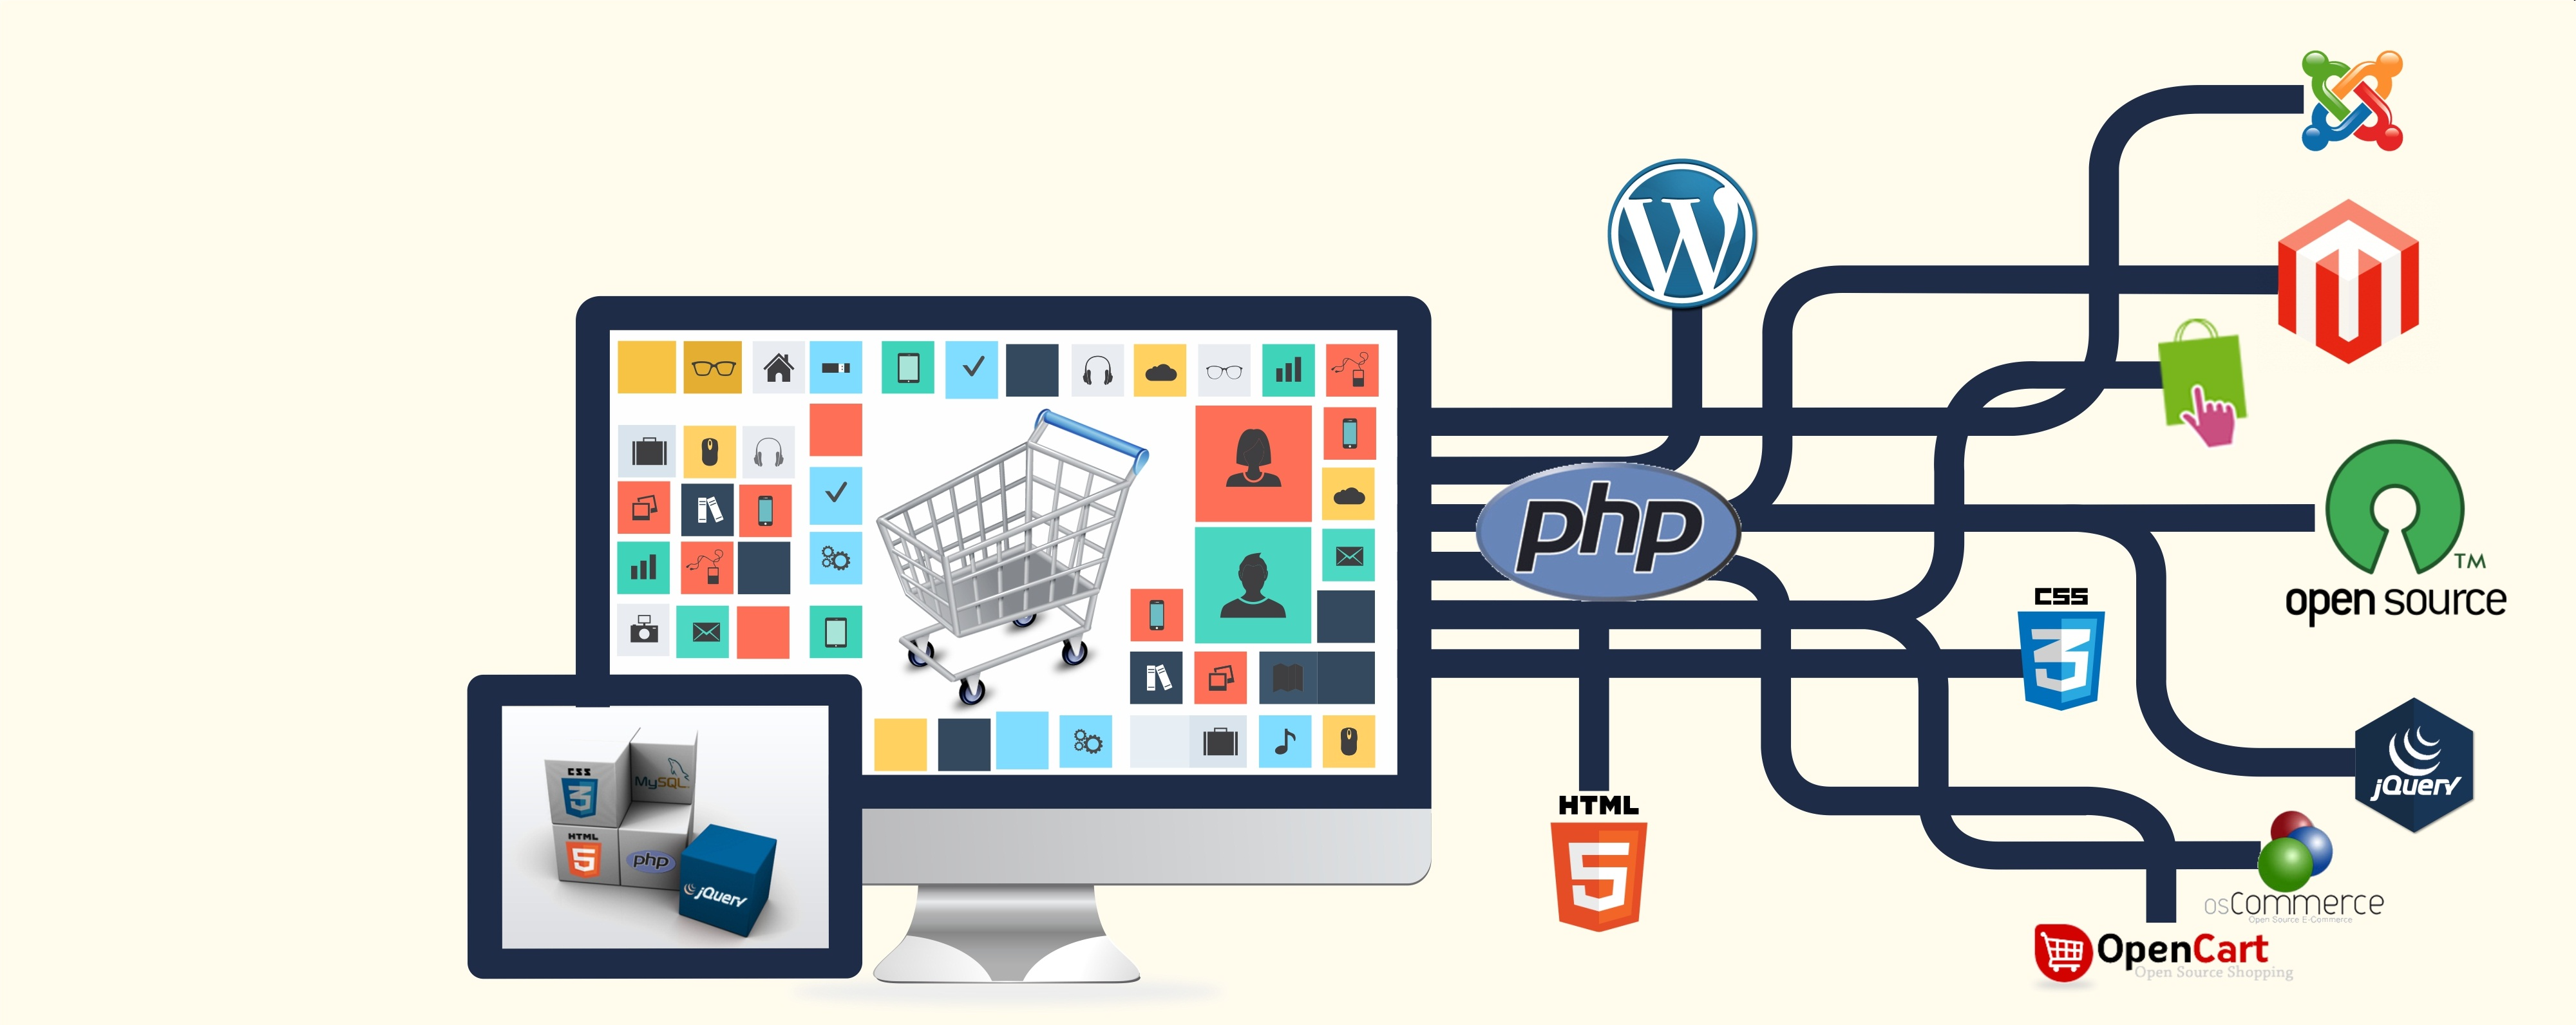
\includegraphics[width=1.0\textwidth]{Images/Research/Technologies/WebTechnologies}
  \caption{Information exchange in an MVC application.} \label{fig:WebTechnologies} 
\end{figure}

There are many web technologies for getting a website up and running, as illustrated in figure \ref{fig:WebTechnologies}. These range from the traditional HTML, CSS, JavaScript and PHP to more modern languages such as Python, Java, and Ruby \cite{Differential:WebTechnologies}. Some of these technologies were researched and have been analysed below as they will most likely be employed for the development process.

\subsubsection{HTML} 
Hyper Text Markup Language (HTML) is a markup language used for structuring and presenting content on the world wide web \cite{W3:HTML5}. HTML 5 is the recommended standard by W3 as of October 28, 2014, and thus will be used to structure the web application being developed. HTML in itself cannot be used to change the style of a page as it was only designed for defining the structure of a page but fortunately, HTML tags can be styled using CSS.

\subsubsection{CSS} 
Cascading Style Sheets (CSS) is a simple mechanism for adding style (e.g. fonts, colours, spacing) to web documents \cite{W3:CSS}. CSS3 is the latest evolution of the Cascading Style Sheets language and aims at extending CSS2.1. It brings a lot of long-awaited novelties, like rounded corners, shadows, gradients, transitions or animations, as well as new layouts like multi-columns, flexible box or grid layouts \cite{Mozilla:CSS3}. CSS3 is being used in this project as it provides a much larger range of styles which are required by Bootstrap.

\subsubsection{JavaScript}
JavaScript (JS) is a high-level, lightweight, interpreted, programming language with first-class functions \cite{Mozilla:JavaScript}. Although JavaScript is not a necessary requirement, it offers many advantages such as allowing manipulation of the document structure after the page has been loaded. As a result of this, one can add, remove or animate content on the page. Inarguably, the main advantage of JavaScript is that it is interpreted on the client-side which means less processing occurs on the server. This allows for faster loading times as parts of the document can be loaded later, on demand, when required. Collectively, all these features, and others not discussed here improve user experience and provide a good reason to incorporate JavaScript into a web application.

\subsubsection{PHP} 
``PHP is a popular general-purpose scripting language that is especially suited to web development'' \cite{PHP:Home}. It is fast, flexible and pragmatic, and powers everything from blogs to the largest and most popular websites in the world \cite{PHP:Home}. One of the main advantages of using PHP is that it allows for untyped variables which are particularly useful for fetching records from the database as the attributes of a tuple will be of different types. Other advantages of PHP include the ability to write Object-Oriented code, particularly useful when implementing the frameworks discussed below.

\subsection{Frameworks}
\begin{figure}[H]
  \centering
  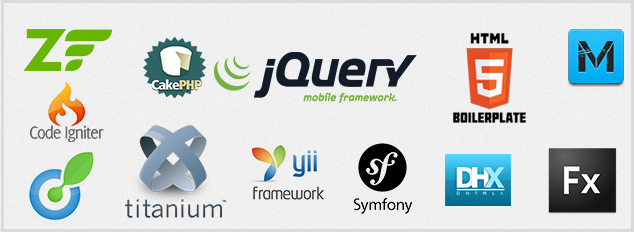
\includegraphics[width=1.0\textwidth]{Images/Research/Technologies/WebFrameworks}
  \caption{Open-source web frameworks built around popular web technologies for developers} \label{fig:WebFrameworks} 
\end{figure}

Frameworks significantly reduce the amount of code that needs to be written to get a project up and running and hence allow the developer to prototype with speed. A range of frameworks are available, as illustrated in figure \ref{fig:WebFrameworks}. Some of these will be employed to develop the project and have been discussed in depth in this section.

\subsubsection{Model-View-Controller (MVC)}
Initially, as stated in the project specification, the system was to be designed as a web-based application implemented using the four basic web technologies mentioned previously in chapter \ref{Section:Web_Technologies}. After completing the initial setup and some implementation, this approach was challenged and a decision was made to find an alternative approach. One of the main reasons for this change in approach was the overwhelming amount of code that was duplicated across pages making it difficult to make changes whilst maintaining consistency across the pages. As a result, it was decided that a Model-View-Controller approach should be used and implemented using an existing framework.

\begin{figure}[H]
  \centering
  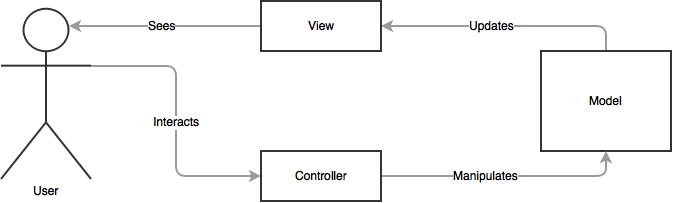
\includegraphics[width=1.0\textwidth]{Images/Research/Technologies/MVC}
  \caption{Information Exchange in an MVC Application.} \label{fig:MVC} 
\end{figure}

The Model-View-Controller (MVC) pattern separates the modelling of the domain, the presentation, and the actions based on user input into three separate classes \cite{MSDN:MVC}. A description of each section as well a graphical representation of communication, available in figure \ref{fig:MVC}, is provided.

\begin{itemize}
    \item \textbf{Model} The model manages the behaviour and data of the application domain, responds to requests for information about its state (usually from the view), and responds to instructions to change state (usually from the controller) \cite{MSDN:MVC}. In essence the model is responsible for all interaction with the database and contains any code that either queries or updates records in the database along with some output formatting.
    \item \textbf{View} The view manages the display of information \cite{MSDN:MVC}. The advantage of this approach is that repeated content can be split into separate views with placeholders and then included by passing in parameters to fill the placeholders. This means that the developers only need to change the code in one place, particularly useful for things such as navigation and footers which are consistent across pages.
    \item \textbf{Controller} The controller interprets the mouse and keyboard inputs from the user, informing the model and view to change as appropriate \cite{MSDN:MVC}. This is where the majority of the logic for the application is written. Any algorithms and data pre or post-processing methods are written inside the controller.
\end{itemize}

\subsubsection{Laravel}
Laravel, an open-source PHP web application framework intended for the development of web applications following the MVC architectural pattern, was chosen after researching various frameworks \cite{Laravel:Home}. Laravel was chosen over other frameworks for a number of reasons - not only does it provide an implementation of the MVC pattern, but it also allows the user to define custom routes and decide where each route leads rather than having the URL be determined by the file path. Additionally, Laravel comes with solutions to a lot of common tasks and problems straight out of the box making it easier to develop the system straight away without having to ``reinvent the wheel''.

\subsubsection{jQuery} 
jQuery is a fast, small, and feature-rich JavaScript library \cite{jQuery:Home}. It will be used over standard JavaScript as it makes tasks like HTML document traversal and manipulation, event handling, animation, and AJAX much simpler with an easy-to-use API that works across a multitude of browsers \cite{jQuery:Home}. Although jQuery does not necessarily provide any additional functionality over JavaScript as it is powered by JavaScript, it provides shorter notations for common JavaScript functions and provides an implementation of features that are lacking in JavaScript, or take long to implement. It can be setup and used by simply including a single script in the document.

\subsubsection{Bootstrap} 
Bootstrap is the most popular HTML, CSS, and JS framework for developing responsive, mobile first projects on the web \cite{Bootstrap:Home}. The main advantage of using Bootstrap is that it easily and efficiently scales your websites and applications with a single code base, from phones to tablets to desktops with CSS media queries. Additionally Bootstrap comes with a whole range of HTML, CSS and jQuery components, that have been pre-styled, further speeding up the development process.

\subsection{Storage}
One of the most fundamental parts of the system is retaining the data that users enter into the system. There are two different storage solutions for storing and querying the data provided by users. These are both discussed below.

\subsubsection{MySQL} 
MySQL is an open-source database management system used for managing data held in a relational database management system (RDBMS) \cite{MySQL:Home}. An SQL database will be used to store all textual information entered by the users. This includes user information, posts, comments, settings and any other necessary information. SQL databases are not encrypted and hence any user credentials such as password will be stored in an encrypted format to prevent access to user accounts in case of a breach.

\subsubsection{Resources}
Along with textual input, it is also necessary to store the images uploaded by the user. One approach to this could be to convert the file to binary and store the binary data in the SQL database. However, this approach would lead to the database rapidly growing in size and in turn affect performance. Not only would queries take longer to execute but this approach would also increase page loading times due to the large record sizes. Another approach would be to store any uploaded files either on a storage server or on the web server so they are available on demand. This would result in faster loading time for pages containing these resources as they do not have to be transferred over the network. Due to this, the latter approach will be used during development.